
\section{Benchmark auf Basis von Interrupts}
\label{chap:benchmark_basis_interrupts}

Der Aufbau der Messmethode basiert auf Softwareinterrupts. Dafür wurde ein eigener Kernelmodul erstellt, der den Benchmark beinhaltet und auf verlangen ausführt.
\par
Ein Interrupt erzwingt den Linux Kernel vom Benutzermodus in den Kernelmodus zu wechseln\cite{Mandl2010_3}. Beim Wechsel werden alle laufende Prozesse zwischen gespeichert, angehalten und anschliessend wird eine Interrupt-Service-Routine (ISR) aufgerufen. Genau diese Eigenschaft wird für den Aufbau der Messmethode verwendet. Den während der Ausführung des ISR sind alle Prozesse angehalten und können der Benchmark der sich selbst in der ISR befindet nicht unterbrechen. Somit wird sicher gestellt das nur der Benchmark ausgeführt und die volle Ressourcen des CPU bekommt bis er fertig ist.
\par
Interrupts sind dafür gemacht, damit sie sofort verarbeitet werden. Ein kleines Beispiel soll dies veranschaulichen. Der Benutzer eines Computer drückt eine Taste auf der Tastatur. Dadurch produziert er ein Hardware-Interrupt. Der aktuelle Prozess wird gespeichert und angehalten. Der Kernel stellt über eine Vektor-Tabelle fest um welchen Interrupt es sich handelt und führt die passende ISR aus, die zur Verarbeitung der gedrückte Tasten dient. ISR sind sehr kurze Programmcodes (Microcode). In diesem Fall speichert der Programmcode die gedrückte Taste in den RAM und übergibt die Ressourcen wieder frei. Der letzte Prozess wird danach, falls er nicht bereits fertig war, weitergeführt. Die Interrupts sind nötig um die Daten am Zeitpunkt des Geschehens zu verarbeiten.
\par
\autoref{fig:Interrupt} beschreibt die unterschiedlichen Interrupts und der Ablauf nach einem eingehender Interrupt. Die Hardware-Interrupts\footnote{Je nach Literatur, Sprache oder Betriebssystem werden unterschiedliche Fachausdrücke verwendet. Der Kontext bleibt aber der selbe.} wurden bereits oben beschrieben. Die "Exception / Trap" sind Interrupts die der CPU selber produziert. Als Beispiel für ein solches Interrupt wäre "Divisions by Zero", wenn man probiert eine Zahl durch Null zu teilen. Die Messmethode in dieser Arbeit stützt sich auf die Software-Interrupts. Software-Interrupts werden häufig verwendet um durch ein Kontextwechsel eine Aufgabe dem Kernel zu übergeben. Durch den Kontextwechsel wird vom unprivilegierten Ring  (Benutzermodus) in den privilegierten Ring (Kernelmodus) gewechselt. Dadurch können auf Befehlssätze und Speicheradressen zugegriffen die im Benutzermodus nicht möglich wären ohne unsicheren Code ausführen zu müssen. Dies wird zum Beispiel notwendig wenn man ein File lesen möchte.

Todo

\begin{figure}[H]
\centering
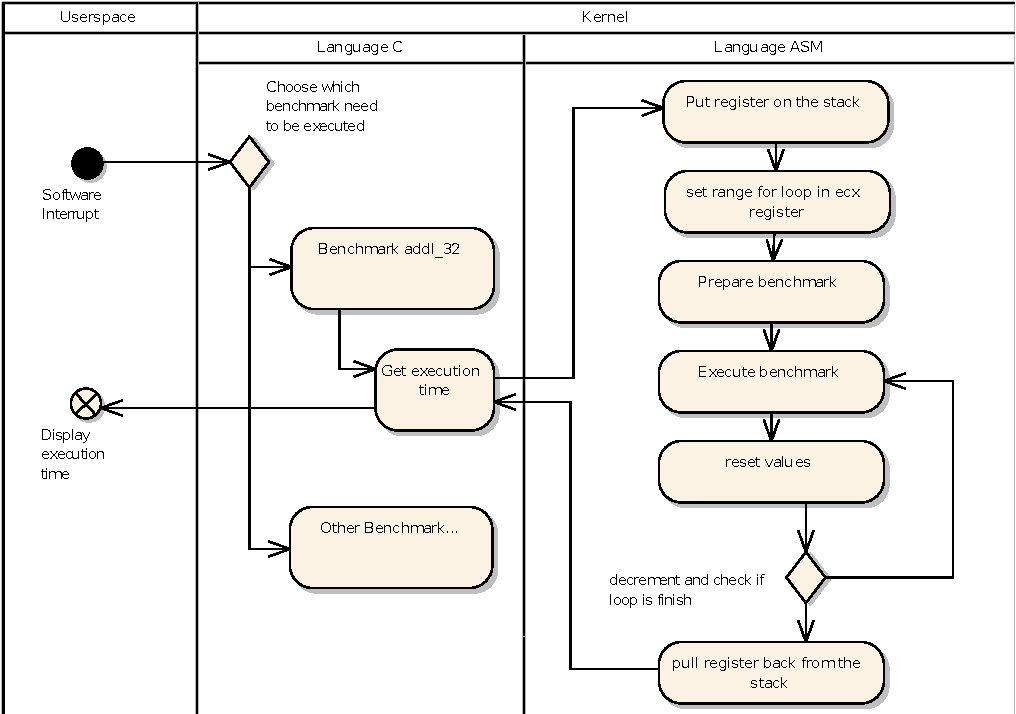
\includegraphics[width=1.0\textwidth]{images/interrupt_ea.pdf}
\caption{Interrupt}
\label{fig:Interrupt}
\end{figure}


\section{Aufbau der Software für die Messung}


\begin{figure}[H]
\centering
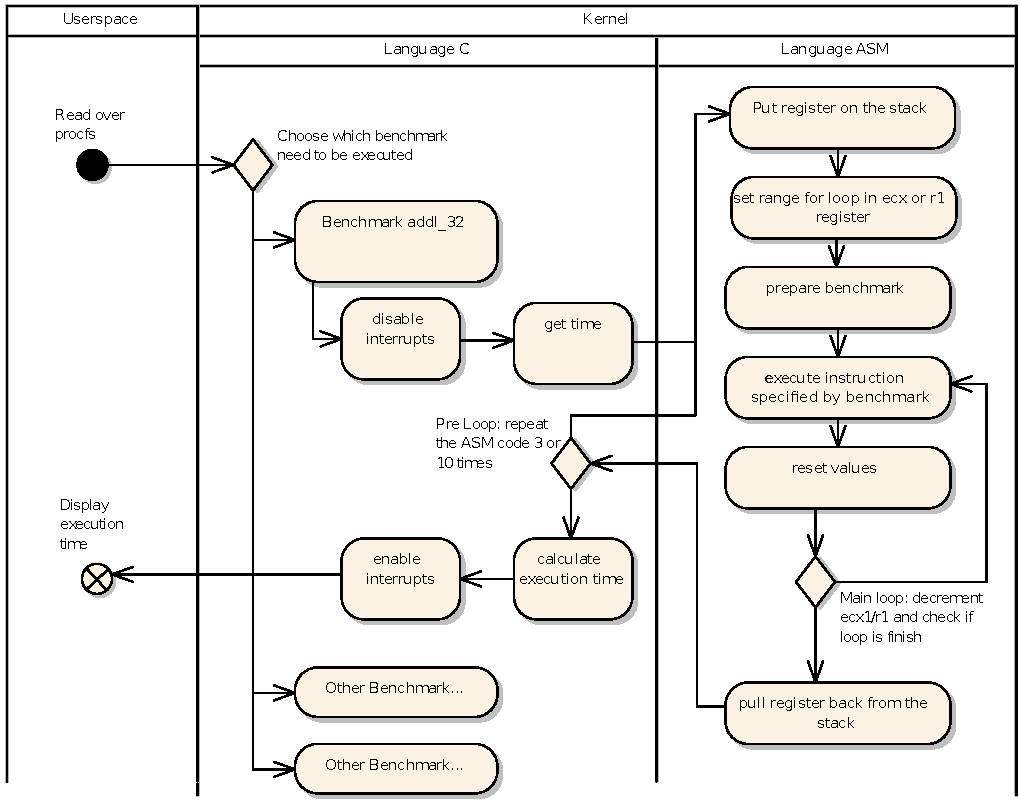
\includegraphics[width=1.0\textwidth]{images/benchmark_ea.pdf}
\caption{Benchmark}
\label{fig:Benchmark}
\end{figure}

